% CT-Meeting 2026 oral presentation.
% Two-channel fidelity for accelerating low-frequency convergence in
% limited-angle DBT PDHG reconstruction.
%
% Build:  latexmk -pdf main.tex   (or pdflatex main.tex 2x for refs)

\documentclass[aspectratio=169,xcolor=dvipsnames]{beamer}

\usepackage[T1]{fontenc}
\usepackage{lmodern}
\usepackage{microtype}
\usepackage{graphicx}
\usepackage{booktabs}
\usepackage{amsmath, amssymb}
\usepackage{tikz}
\usetikzlibrary{positioning, arrows.meta, fit}
\usepackage{xcolor}

\graphicspath{{figs/}}

% Tolerate up to 20pt vertical overflow before warning. Metropolis's
% title page minipage and a few content-rich slides report residual
% \vfill space as overflow even though nothing is visually clipped;
% real overflows on this deck are >20pt and still get caught.
\vfuzz=20pt

% Theme ---------------------------------------------------------------
\usetheme{metropolis}
\metroset{sectionpage=none}
\setbeamertemplate{frame numbering}[fraction]
\definecolor{MainAccent}{HTML}{1F4E79}
\definecolor{SubAccent}{HTML}{C00000}
\setbeamercolor{frametitle}{bg=MainAccent, fg=white}
\setbeamercolor{progress bar}{fg=MainAccent}
\setbeamercolor{title separator}{fg=MainAccent}

% Section badge: short section name shown in the top-right of every
% frame with a frametitle. Uses an absolute TikZ overlay so it does not
% interfere with the metropolis frametitle bar.
\addtobeamertemplate{frametitle}{}{%
  \begin{tikzpicture}[remember picture, overlay]
    \node[anchor=north east, inner xsep=0.35cm, inner ysep=0.22cm,
          text=white, font=\scriptsize\itshape, opacity=0.85]
      at (current page.north east) {\insertsectionhead};
  \end{tikzpicture}%
}

% Title ---------------------------------------------------------------
% Tighten the metropolis title page: with 6 authors on 2 lines and 5
% institutions on 2 lines, the default templates overflow by ~16pt.
% Override the author/institute templates to use smaller fonts and less
% vertical padding so everything fits.
\setbeamerfont{author}{size=\footnotesize}
\setbeamerfont{institute}{size=\scriptsize}
\setbeamerfont{date}{size=\footnotesize}
\setbeamertemplate{author}{%
  \vspace*{1em}\insertauthor\par\vspace*{0.15em}}
\setbeamertemplate{institute}{%
  \vspace*{1mm}\insertinstitute\par}
\title{Accelerating Low-Frequency Convergence for Limited-Angle Reconstruction (LAR)}
\subtitle{Two-Channel Fidelity in PDHG}
\author[Iyadomi]{%
  Taro Iyadomi\inst{1,6} \and
  Ricardo Parada\inst{2,6} \and
  Anna Kim\inst{3,6} \and
  Lily Jiang\inst{4,6} \and
  Emil Sidky\inst{5} \and
  William Chang\inst{4,6}}
\institute[]{%
  \inst{1}Northwestern University \quad
  \inst{2}UC Riverside \quad
  \inst{3}UC San Diego \and
  \inst{4}UC Los Angeles \quad
  \inst{5}University of Chicago \quad
  \inst{6}BruinML}
\date{CT Meeting 2026}

% Macros --------------------------------------------------------------
\newcommand{\Rhi}{R_{\mathrm{hi}}}
\newcommand{\Rlo}{R_{\mathrm{lo}}}
\newcommand{\Hann}{\mathrm{Hann}^{1/2}}

% Figure helpers: width-limited but height-capped so a caption / bullets
% always fit on the slide. Optional first arg = height cap (frac of text).
\newcommand{\deckfig}[2][0.70]{%
  \includegraphics[width=\linewidth,height=#1\textheight,keepaspectratio]{#2}}

% Small italic "how it was generated" note pinned to each figure slide.
\newcommand{\geomnote}[1]{\par\smallskip{\scriptsize\itshape #1}}

\begin{document}

% =========================================================================
\begin{frame}[plain]
  \titlepage
\end{frame}

% =========================================================================
\section[Motivation]{Motivation}
% =========================================================================

\begin{frame}{What is limited-angle reconstruction?}
  \begin{itemize}
    \item Tomography recovers a cross-section by computing line
          integrals of X-ray beams from many source positions around
          the object.
    \item \textbf{Sufficient sampling.} For a fan-beam scan, a source
          arc of $180^{\circ}$ plus the fan angle is already a complete
          measurement set; everything past that just re-measures the
          same rays from the other side.
    \item \textbf{Limited-angle reconstruction (LAR)} uses a source arc
          \emph{strictly below} that threshold. A wedge of spatial
          frequencies is never measured, and the inverse problem is no
          longer determined by the data alone.
    \item \textbf{Digital breast tomosynthesis (DBT)} is the clinical
          setting we focus on. With a source arc of only
          $[15^{\circ}, 50^{\circ}]$, the reconstruction is severely
          ill-posed.
  \end{itemize}
\end{frame}

\begin{frame}{Why DBT?}
  \begin{itemize}
    \item Annual mammographic screening is the standard of care for
          breast cancer --- \textbf{$\approx\!43$ million screenings
          per year in the US.}\textsuperscript{1}
    \item Standard mammography is a single 2D projection. Overlapping
          fibroglandular (``dense'') tissue can mask small lesions.
          \textbf{$\approx\!40\%$ of screening-age women have dense
          breasts}\textsuperscript{2}, and density is itself a risk
          factor ($\approx\!2\times$ cancer risk for extremely dense
          vs scattered).\textsuperscript{3}
    \item \textbf{DBT.} Short-arc sweep $\rightarrow$ quasi-3D volume:
          depths separate, lesion conspicuity improves. Validated as a
          viable replacement for full-field digital
          mammography.\textsuperscript{4}
    \item \textbf{Dose.} An annual exam $\Rightarrow$ low-dose
          acquisition: few views, short arc.
  \end{itemize}
  \vspace{0.8em}
  {\scriptsize
  \textsuperscript{1}\,FDA MQSA National Statistics, 2025 Scorecard.\\
  \textsuperscript{2}\,Society of Breast Imaging,
    \emph{Breast Density and Supplemental Screening}.\\
  \textsuperscript{3}\,Bodewes et al., \emph{The Breast} 66:62--68, 2022.\\
  \textsuperscript{4}\,A.\,Badano et al., \emph{JAMA Netw.\ Open}
    1(7):e185474, 2018.\par}
\end{frame}

\begin{frame}{DBT geometry and acquisition}
  \begin{columns}[T,onlytextwidth]
    \column{.55\textwidth}
    \begin{itemize}
      \item \textbf{Geometry.} The breast is compressed between the
            detector and a paddle; the X-ray tube sweeps a short arc
            above. A full gantry rotation is mechanically impossible.
      \item \textbf{Acquisition time.} A short sweep is fast, limiting
            motion blur from breathing and patient discomfort under
            compression.
      \item \textbf{Beyond DBT.} The same constraints --- restricted
            mechanical access, short scan time --- appear in lung-nodule
            and kidney-stone imaging.
    \end{itemize}
    \column{.45\textwidth}
    \centering
    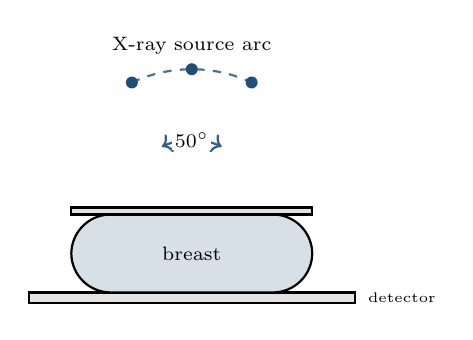
\begin{tikzpicture}[scale=0.9, every node/.style={font=\scriptsize}]
      % Detector (gray bar at the bottom)
      \draw[fill=gray!22, thick] (-2.3, -1.30) rectangle (2.3, -1.15);
      \node[anchor=west, font=\tiny] at (2.35, -1.22) {detector};
      % Breast: compressed shape -- flat top/bottom (against paddle and
      % detector), rounded sides. Implemented as a rounded rectangle.
      \draw[fill=MainAccent!18, thick, rounded corners=0.50cm]
        (-1.7, -1.15) rectangle (1.7, -0.05);
      \node at (0, -0.60) {breast};
      % Top compression paddle (thin gray bar above the breast)
      \draw[fill=gray!22, thick] (-1.7, -0.05) rectangle (1.7, 0.05);
      % Source arc (dashed) above the paddle
      \draw[dashed, thick, MainAccent!80]
        (115:2.0) arc[start angle=115, end angle=65, radius=2.0];
      \node[above=2pt] at (90:2.0) {X-ray source arc};
      % Three source positions
      \foreach \a in {115, 90, 65} {
        \fill[MainAccent] (\a:2.0) circle (2.4pt);
      }
      % Angle indicator (curved double-arrow) for the angular wedge
      \draw[<->, MainAccent!90, thick]
        (115:1.0) arc[start angle=115, end angle=65, radius=1.0];
      \node[fill=white, inner sep=1pt] at (90:1.0) {$50^{\circ}$};
    \end{tikzpicture}
  \end{columns}
\end{frame}

\begin{frame}{Why LAR is hard}
  \centering
  \small
  \[
    \min_{f \geq 0}\;
      \underbrace{\alpha_x\|\partial_x f\|_1
                + \alpha_y\|\partial_y f\|_1
                + \alpha_z\|\partial_z f\|_1}_{\text{directional TV (smoothness)}}
    + \underbrace{\beta\|f\|_1}_{\text{pixel sparsity}}
  \]
  \vspace{-0.7em}
  \[
    \text{s.t.}\quad
      \underbrace{\|g - Xf\|_2 \leq \varepsilon\sqrt{\mathrm{size}(g)}}_{\text{data-fidelity ball}}
  \]
  \normalsize
  \begin{itemize}\setlength\itemsep{0pt}
    \item \textbf{Severely under-determined.} Unknowns exceed
          measurements by an order of magnitude or more --- and the
          gap widens in 3D ($N^{3}$ vs $N^{2}$).
  \end{itemize}
  \begin{center}
    \scriptsize
    \renewcommand{\arraystretch}{0.8}
    \begin{tabular}{lcc}
      \toprule
      Slice resolution & Unknowns (pixels) & Measurements (rays) \\
      \midrule
      $512^2$ & $262{,}144$ & $25{,}600$ \\
      $256^2$ & $65{,}536$  & $25{,}600$ \\
      $128^2$ & $16{,}384$  & $25{,}600$ \\
      \bottomrule
    \end{tabular}\par\smallskip
    $25$ \emph{views} $\times$ $1024$ \emph{bins} per view.
  \end{center}
\end{frame}

% =========================================================================
\section[Setup]{The reconstruction setup}
% =========================================================================

\begin{frame}{Reconstruction with PDHG (Chambolle--Pock)}
  \textbf{What this kind of problem needs from an optimizer:}
  \begin{itemize}\setlength\itemsep{0pt}
    \item Handle non-smooth terms ($\ell_1$, TV --- no usable gradient).
    \item Handle hard constraints (data-fidelity ball, $f \geq 0$).
    \item Scale to millions of unknowns; matrix factorization is out.
  \end{itemize}
  \medskip
  \textbf{Primal--dual hybrid gradient} (PDHG / Chambolle--Pock, 2011)
  alternates a \emph{dual} step (project onto the data ball) with a
  \emph{primal} step (proximal map for $\ell_1$/TV $+$ non-negativity).
  Each iteration: a matrix-vector product, a projection, a prox.
  No derivatives, no inverses.
\end{frame}

\begin{frame}{Single-channel data fidelity}
  Sidky et al.\footnote{E.\,Y.\,Sidky et al., \emph{J.\ Med.\ Imaging}
  12(S1):S13013, 2025.} promote the plain residual in the data-fidelity
  constraint to a square-root Hann-weighted residual:
  \[
    \|g - Xf\|_2 \leq \varepsilon\sqrt{\mathrm{size}(g)}
    \quad\longrightarrow\quad
    \|R_{[c]}(g - Xf)\|_2 \leq \varepsilon\sqrt{\mathrm{size}(g)}.
  \]
  \vspace{-0.8em}
  \begin{itemize}\setlength\itemsep{0pt}
    \item \textbf{$R_{[c]} = \Hann(c)$} attenuates low spatial
          frequencies in the residual --- robust to low-frequency noise
          streaks.
    \item PDHG with He--Yuan over-relaxation, $\rho \approx
          1.75$.\footnote{B.\,He, X.\,Yuan, \emph{SIAM J.\ Imag.\ Sci.}
          5(1):119--149, 2012.}
  \end{itemize}
  \textbf{Single-channel:} one weighted residual covers the whole
  frequency spectrum.
\end{frame}

% =========================================================================
\section[Bottleneck]{The problem}
% =========================================================================

\begin{frame}{What happens during a single-channel run}
  \centering
  \deckfig[0.60]{single_only_ladder_256_paper.png}
  \vspace{0.3em}
  \begin{itemize}\setlength\itemsep{0pt}\small
    \item Fine structure (calcifications, glandular speckling) settles fast.
    \item Large soft-tissue regions stay blurred, with a slowly-varying
          intensity error, through iter ${\sim}100\text{--}300$.
    \item This is the low-frequency convergence bottleneck.
  \end{itemize}
  \geomnote{2D fan-beam $\cdot$ 25 views $\cdot$ 50$^\circ$ arc $\cdot$ $256^2$ grid}
\end{frame}

\begin{frame}{Why does this happen?}
  \textbf{Stability:}\;
  $\tau \sigma \|R_{[c]}X\|^2 < 1 \;\Longrightarrow\; \sigma < \dfrac{1}{\tau\,s_{\max}^2}$
   (step size capped by the largest singular value)

  \medskip
  \textbf{Per-mode correction $\propto \sigma \cdot s_k^2$.}
  With $\sigma$ pinned to its bound:
  \begin{itemize}\setlength\itemsep{0pt}
    \item High-$k$ (large $s_k$): stronger drive, faster convergence.
    \item Low-$k$ (small $s_k$): weaker drive, slower convergence.
  \end{itemize}

  \medskip
  \textbf{Two effects compound at low $k$:}
  \begin{itemize}\setlength\itemsep{0pt}
    \item \emph{LAR geometry}: $s_k$ already tiny (ill-conditioning).
    \item \emph{Hann filter}: shrinks low-$k$ $s_k$ further (noise
          suppression).
  \end{itemize}
\end{frame}

% =========================================================================
\section[Two-channel]{The idea: two-channel fidelity}
% =========================================================================

\begin{frame}{Two-channel data fidelity}
  \centering
  \small
  \[
    \min_{f \geq 0}\;
    \alpha_i \|\partial_i f\|_1 + \beta \|f\|_1
    \quad \text{s.t.}\quad
    \begin{cases}
      \|\Rhi(g - Xf)\|_2 \le \varepsilon_{\mathrm{hi}}\sqrt{\mathrm{size}(g)} \\[2pt]
      \|\Rlo(g - Xf)\|_2 \le \varepsilon_{\mathrm{lo}}\sqrt{\mathrm{size}(g)}
    \end{cases}
  \]
  \normalsize
  \vspace{0.3em}

  \resizebox{\textwidth}{!}{%
  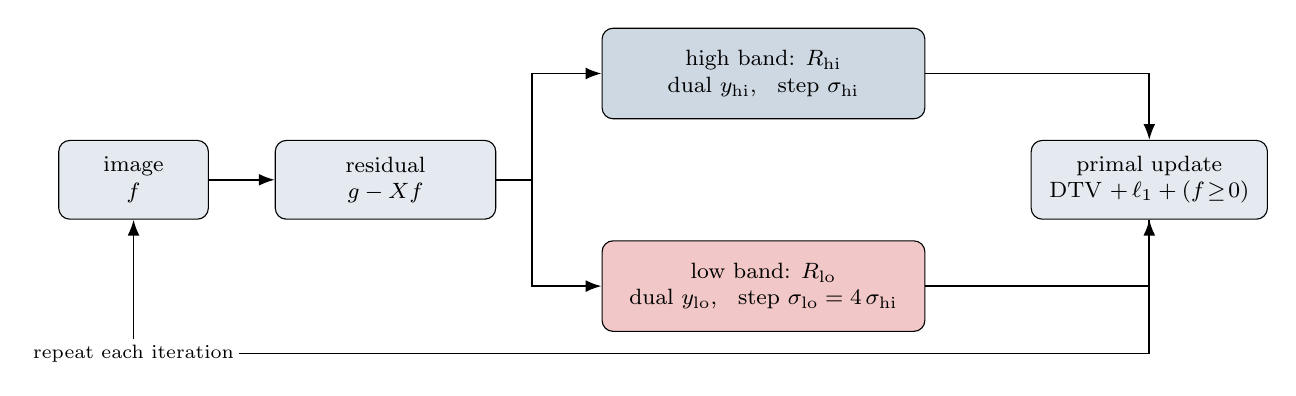
\begin{tikzpicture}[
    every node/.style={font=\footnotesize},
    box/.style={draw, rounded corners, align=center, fill=MainAccent!12,
                minimum height=1.0cm},
    hi/.style={draw, rounded corners, align=center, fill=MainAccent!22,
               minimum height=1.15cm, minimum width=4.1cm},
    lo/.style={draw, rounded corners, align=center, fill=SubAccent!22,
               minimum height=1.15cm, minimum width=4.1cm},
    arr/.style={-Latex, semithick},
  ]
    \node[box, minimum width=1.9cm] (img)  at (0,0)     {image\\$f$};
    \node[box, minimum width=2.8cm] (res)  at (3.2,0)   {residual\\$g - X f$};
    \node[hi]                       (hi)   at (8.0,1.35)
      {high band: $\Rhi$\\dual $y_{\mathrm{hi}}$,\;\; step $\sigma_{\mathrm{hi}}$};
    \node[lo]                       (lo)   at (8.0,-1.35)
      {low band: $\Rlo$\\dual $y_{\mathrm{lo}}$,\;\; step $\sigma_{\mathrm{lo}} = 4\,\sigma_{\mathrm{hi}}$};
    \node[box, minimum width=3.0cm] (prim) at (12.9,0)
      {primal update\\DTV $+\,\ell_1+ (f\!\ge\!0)$};

    \draw[arr] (img) -- (res);
    \draw[arr] (res.east) -- ++(0.45,0) |- (hi.west);
    \draw[arr] (res.east) -- ++(0.45,0) |- (lo.west);
    \draw[arr] (hi.east) -| (prim.north);
    \draw[arr] (lo.east) -| (prim.south);
    \draw[arr] (prim.south) -- ++(0,-1.7) -| (img.south)
      node[pos=0.5, fill=white, inner sep=2pt, font=\scriptsize]
        {repeat each iteration};
  \end{tikzpicture}}
\end{frame}

% =========================================================================
\section[Results]{Results}
% =========================================================================

% 2D paper breast -----------------------------------------------------

\begin{frame}{2D fan-beam: single vs two-channel}
\footnotesize\itshape 2D fan-beam first as proof-of-concept; 3D cone-beam phantoms follow.\normalfont\normalsize

  \centering
  \deckfig[0.50]{iter_ladder_recon_256_paper.png}
  \vspace{0.2em}
  \begin{itemize}\setlength\itemsep{0pt}\small
    \item Two-channel resolves recognizable soft-tissue structure
          several iterations earlier than single-channel.
  \end{itemize}
  \geomnote{2D fan-beam $\cdot$ 25 views $\cdot$ 50$^\circ$ arc $\cdot$ $256^2$ grid}
\end{frame}

\begin{frame}{Convergence behaviour}
  \centering
  \deckfig[0.58]{iter_ladder_convergence_256_paper.png}
  \begin{itemize}\setlength\itemsep{0pt}\small
    \item Single-channel oscillates strongly through iter ${\sim}200$;
          two-channel converges smoothly from the start.
  \end{itemize}
  \geomnote{2D fan-beam $\cdot$ 25 views $\cdot$ 50$^\circ$ arc $\cdot$ $256^2$ grid}
\end{frame}

\begin{frame}{Persistence across image sizes}
  \centering
  \deckfig[0.55]{persistence_500iter.png}
  \begin{itemize}\setlength\itemsep{0pt}\small
    \item Two-channel sits below single-channel at every resolution.
    \item Iter-$500$ image-RMSE reduction: $19\%$, $22\%$, $62\%$ at
          $512^{2}$, $256^{2}$, $128^{2}$.
  \end{itemize}
  \geomnote{2D fan-beam $\cdot$ 25 views $\cdot$ 50$^\circ$ arc $\cdot$ $512^2$, $256^2$, $128^2$ grids}
\end{frame}

% 2D Shepp-Logan -- generality check ----------------------------------

\begin{frame}{2D Shepp--Logan: generality check}
  \centering
  \deckfig[0.58]{shepp_logan_2d_iter_ladder.png}\\[0.3em]
  \footnotesize
  Same 2D fan-beam setup, same hyperparameters, standard
  Shepp--Logan phantom. Two-channel resolves the interior ellipses
  earlier; iter-$500$ image-RMSE $9\%$ below single-channel
  ($0.078$ vs.\ $0.086$).
  \geomnote{2D fan-beam $\cdot$ 25 views $\cdot$ 50$^\circ$ arc $\cdot$ $256^2$ grid}
\end{frame}

% 3D synthetic breast phantom -----------------------------------------

\begin{frame}{3D synthetic breast: iteration ladder}
  \centering
  \deckfig[0.60]{ct2_breast_synthetic_A_powerlaw_iter_ladder.png}\\[0.3em]
  \footnotesize
  Mid-axial slice across iterations. Two-channel resolves the dense
  glandular regions earlier and avoids the dark wedge artifact that
  develops in single-channel from iter ${\sim}50$ onward.
  \geomnote{3D cone-beam $\cdot$ 25 views $\cdot$ 15$^\circ$ arc $\cdot$ $432\times432\times96$ grid}
\end{frame}

\begin{frame}{3D synthetic breast: convergence}
  \centering
  \deckfig[0.60]{ct2_breast_synthetic_A_powerlaw_convergence.png}\\[0.3em]
  \footnotesize
  Image RMSE vs.\ iteration. Two-channel diverges from single-channel
  after iter ${\sim}20$ and maintains a clear gap; iter-$100$ RMSE
  reduction is ${\sim}33\%$ ($0.033$ vs.\ $0.049$).
  \geomnote{3D cone-beam $\cdot$ 25 views $\cdot$ 15$^\circ$ arc $\cdot$ $432\times432\times96$ grid}
\end{frame}

% Slide A: formulation -------------------------------------------------
\begin{frame}{Extension: coupled multi-fidelity formulation}
  \renewcommand{\thempfootnote}{\arabic{mpfootnote}}
  \footnotesize
  Sidky et al.\ (2026) extend the multi-fidelity idea to wide-angle
  clinical DBT, reconstructing \emph{three} coupled
  images:\footnote[1]{E.\,Y.\,Sidky et al., arXiv:2605.29133, 2026.}
  \[\small
  \begin{aligned}
    \min_{f_1,f_2,f_3}\;\;
      & \sum_{i \in \{x,y,a,b\}}\!\!\alpha_i\bigl(\|\partial_i f_1\|_1 + \|\partial_i f_2\|_1\bigr)
        + \alpha_1\bigl(\|f_1\|_1 + \|f_2\|_1\bigr) + \alpha_3 \|f_3\|_1 \\
    \text{s.t.}\;\;
      & f_1 - f_2 = f_3, \\
      & \|R_{[c]}(X G_{[d_1]} f_1 - g)\|_2 \le \varepsilon_1 \sqrt{N_{\mathrm{data}}}, \\
      & \|R_{[c]}(X G_{[d_2]} f_2 - G^{\mathrm{det}}_{[d_d]} g)\|_2 \le \varepsilon_2 \sqrt{N_{\mathrm{data}}}.
  \end{aligned}
  \]
  \vspace{-0.4em}
  \begin{itemize}\setlength\itemsep{1pt}
    \item $f_1$: standard recon; $f_2$: smooth background; $f_3 = f_1 - f_2$ displayed.
    \item Two data-fidelity terms with different Gaussian blurs $G_{[d_1]}, G_{[d_2]}$
          span low- and high-frequency bands.
    \item Same multi-fidelity insight, different construction. 
  \end{itemize}
\end{frame}

% Slide B: f1/f2/f3 separation ------------------------------------------
\begin{frame}{Coupled recon: $f_1$, $f_2$, $f_3$ separation}
  \centering
  \deckfig[0.78]{sidky_coupled_f1f2f3.png}\\[0.1em]
  \footnotesize
  Left to right: $f_1$, $f_2$ smooth background, $f_3 = f_1 - f_2$ (display).
  Profile along the dashed line: $f_2$ (dashed) tracks the slow background
  drift while $f_1$ (solid) retains structural detail.
\end{frame}

% Slide C: clinical comparison ------------------------------------------
\begin{frame}{Coupled recon: patient-case comparison}
  \renewcommand{\thempfootnote}{\arabic{mpfootnote}}
  \begin{columns}[T,onlytextwidth]
    \column{.42\textwidth}
    \footnotesize
    Coupled DTV-LSQ (with background absorbed by $f_2$), compared against
    a zero-initialized LSQ-Tik baseline on a real patient case.\footnote{E.\,Y.\,Sidky
    et al., arXiv:2605.29133, 2026.}
    \medskip

    \begin{itemize}\setlength\itemsep{2pt}
      \item Tighter grayscale window: low-frequency background artifacts
            absorbed by $f_2$.
      \item Sharper depth resolution from DTV initialization.
      \item Mass near the chest wall is more conspicuous.
    \end{itemize}
    \column{.58\textwidth}
    \deckfig[0.65]{sidky_dtvinit_vs_zeroinit.png}\\
    \centering
    {\scriptsize\itshape DTVinit-LSQ-Tik (left) vs.\ zero-init baseline
    (right).\\Wide-angle $50^\circ$ Siemens Mammomat B.brilliant.}
  \end{columns}
\end{frame}

% =========================================================================
\section[Conclusion]{Conclusion}
% =========================================================================

\begin{frame}{Summary}
  \begin{itemize}
    \item LAR reconstruction has a \emph{mode-dependent} convergence
          bottleneck: low spatial frequencies are starved of corrective
          drive because the PDHG step size is bound by high-frequency
          stability.
    \item Splitting the data fidelity into a low-pass and a high-pass
          channel, each with its own dual variable and step size,
          accelerates low-frequency settling without breaking stability.
    \item Confirmed on a 2D breast phantom ($26\%$ iter-$100$ RMSE
          reduction at $50^\circ$ arc), on Shepp--Logan (generality),
          and on a 3D synthetic breast at $15^\circ$ DBT arc
          ($33\%$ iter-$100$ reduction).
  \end{itemize}
\end{frame}

\begin{frame}{Future work}
  \begin{itemize}
    \item \textbf{Why just two channels?} Extend the two-band split to a
          multi-channel band-pass decomposition. More channels could
          give finer per-mode control, at the cost of additional dual
          variables and a more careful step-size schedule.
    \item \textbf{Convergence guarantees.} Derive the per-band step
          sizes from a theoretical analysis that connects the empirical
          step-size heuristic to established PDHG convergence theory.
    \item \textbf{Tuning the low-frequency constraint.} The per-band
          data-tolerance ratio that minimises image RMSE is not the
          same on 2D and 3D phantoms. Understanding what problem
          features control it is open.
  \end{itemize}
\end{frame}

\begin{frame}[standout]
  Thank you!
\end{frame}

% =========================================================================
\appendix
% =========================================================================

\begin{frame}{References}
  \footnotesize
  \begin{itemize}
    \item E.\,Y.\,Sidky et al., \emph{Accurate volume image reconstruction for
          DBT with directional-gradient and pixel sparsity regularization},
          J. Med. Imaging 12(S1):S13013, 2025.
    \item E.\,Y.\,Sidky, A.\,A.\,Sanchez, J.\,P.\,Phillips, Z.\,Zhang,
          D.\,Xia, I.\,S.\,Reiser, X.\,Pan, \emph{Improving
          depth-resolution, in-plane contrast, and reducing
          non-uniformity artifacts for wide-angle DBT},
          arXiv:2605.29133, 2026.
    \item A.\,Chambolle, T.\,Pock, \emph{A first-order primal-dual algorithm
          for convex problems with applications to imaging},
          J. Math. Imag. Vision 40(1):120--145, 2011.
    \item B.\,He, X.\,Yuan, \emph{Convergence analysis of primal-dual
          algorithms for a saddle-point problem: from contraction perspective},
          SIAM J. Imag. Sci. 5(1):119--149, 2012.
    \item Z.\,Zhang, B.\,Chen, D.\,Xia, E.\,Y.\,Sidky, X.\,Pan,
          \emph{Directional-TV algorithm for image reconstruction from
          limited-angular-range data}, Med. Image Anal. 70:102030, 2021.
    \item A.\,Badano et al., \emph{Evaluation of digital breast
          tomosynthesis as replacement of full-field digital mammography
          using an in silico imaging trial}, JAMA Netw. Open
          1(7):e185474, 2018.
    \item F.\,T.\,H.\,Bodewes, A.\,A.\,van Asselt, M.\,D.\,Dorrius,
          M.\,J.\,W.\,Greuter, G.\,H.\,de Bock, \emph{Mammographic
          breast density and the risk of breast cancer: a systematic
          review and meta-analysis}, The Breast 66:62--68, 2022.
  \end{itemize}
\end{frame}

\end{document}
